\chapter{Shell Balances}

The goal of this chapter is to establish a method for determining the velocity, temperature and concentration profiles in a fluid system by balancing momentum across a thin "shell" in space and then integrating across all shells of the same shape.

We apply these balances to understand how the equations for the velocity profile of these systems are developed and to build a good intuition for the behaviour of these transport properties in various systems.

\section{Shell Momentum Balances}

In this section, we will be looking at how to derive the following in various geometries :

\begin{itemize}

    \item Velocity profiles for laminar flows ($v_{x}$, $v_{y}$, $v_{z}$)

    \item Momentum flux profiles ($\tau_{ij}$)

    \item Maximum velocity, average velocity and shear stress

\end{itemize}


The momentum balance equation across a thin shell is as such: \{Rate of combined momentum flux in\} - \{Rate of combined momentum flux out\} + \{forces acting on the system\} = 0


\subsection{Shell Momentum Balance Algorithm:}

\begin{enumerate}

    \item \textbf{Identify non-vanishing terms:} Several problems are 1 or 2 dimensional, in which case there may be no flow in certain directions. e.g. : $v_{x} = 0$, which immediately reduces a lot of equations. Another example: if $v_{x}$ is only a function of y then all terms such as $\frac{\partial v_{x}}{\partial x}$ and $\frac{\partial v_{x}}{\partial z}$ disappear immediately.

    \item \textbf{Write the momentum balance over a thin shell perpendicular to spatial variables:} This thin shell may have $\Delta x$, $\Delta y$ or $\Delta z$ terms and is perpendicular to the directions of momentum transport.

\item \textbf{Thickness of the shell tending to zero:} By taking limits tending to zero, the momentum balance equations become differential equations for momentum flux. For example, \[\lim_{\Delta x \to 0} \frac{\tau(x+\Delta x) - \tau(x)}{\Delta x} = \frac{\partial \tau}{\partial x}\]

    \item \textbf{Integrate the differential equations:} Integrating the first order equation in $\tau$ derives the momentum flux distribution.

    \item \textbf{Apply Newton's Law of Viscosity:} This converts the momentum flux expression into a first order differential equation in terms of velocity.

    \item \textbf{Derive the velocity profile:} Integrate the differential equation in terms of velocities to obtain the velocity profile of the system.

    \item \textbf{Apply Boundary Conditions:} The boundary conditions give us the values for the constants of integration in the above expressions.

\end{enumerate}

\subsection{Boundary Conditions in Momentum Transport}

\begin{itemize}

    \item Solid-Fluid Interface: No-slip boundary condition. We assume that the velocity of a fluid at the point of contact with a solid is that same as the velocity of the solid.

    \item Liquid-Liquid Interface: At the interface of two immiscible liquids, we assume that there is no discontinuity in the velocity. We also take the value of momentum flux to be the same at the interface.

    \item Liquid-Gas Interface: We assume that flowing liquids do not impart any momentum onto a gas at a liquid-gas interface.

\end{itemize}


\subsection{Illustrative Problems}

\subsubsection{Flow of a Falling Film}

Assume we have a liquid flowing down an inclined plate as shown in the figure below. The liquid film on top of the inclined plate has a small thickness $\delta$, which is much smaller than the dimensions of the plate (W, L). 

\begin{figure}[h]
    \centering
    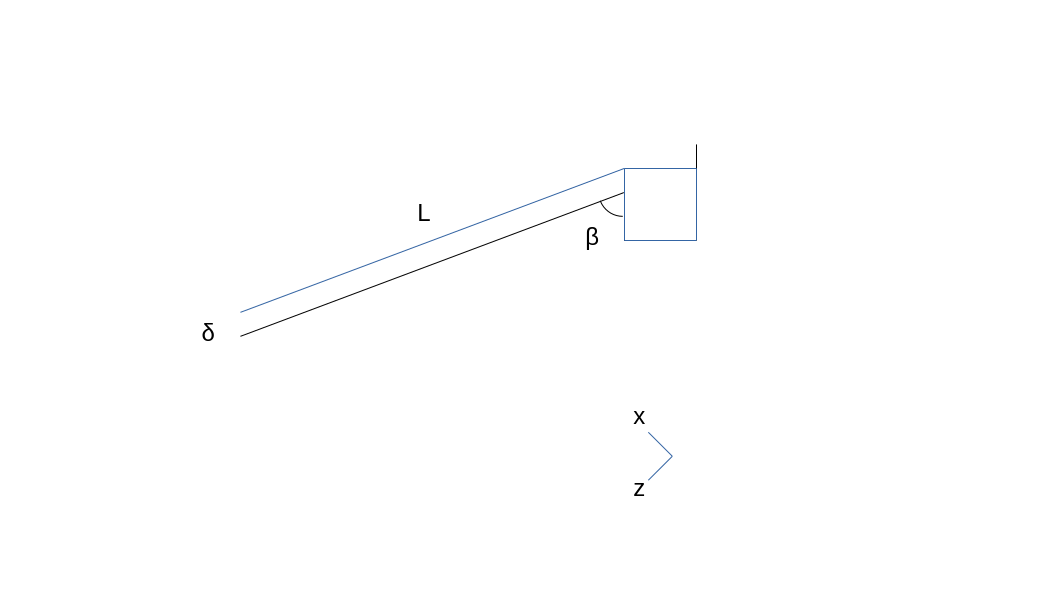
\includegraphics[scale=0.45]{figure_fall}
    \caption{Falling Film Problem}
\end{figure}

To assess the velocity profile of the liquid from the surface of the plate to the surface of the film, we will apply the method of shell momentum balances as prescribed in the algorithm above.


\begin{itemize}

    \item Since the velocity is only in the z direction, the terms $v_{x}$ and $v_{y}$ become 0. The shell momentum balances hence only consider the terms of the momentum flux tensor that impart z-momentum, which are $\phi_{xz}$, $\phi_{yz}$ and $\phi_{zz}$. 

    \item The velocity profile changes only in the x direction, since W and L are significantly larger than $\delta$. $\frac{\partial v_{z}}{\partial y}$ and $\frac{\partial v_{z}}{\partial z}$ are 0.

    \item The differential slice $\Delta x$ considered is a thin slice somewhere between x = 0 and x = $\delta$.

    \item Recall $$\phi_{zz} = \rho v_{z} v_{z} + \tau_{zz} + P ,$$ $$\phi_{xz} = \rho v_{x} v_{z} + \tau_{xz} ,$$ $$\phi_{yz} = \rho v_{y} v_{z} + \tau_{yz}$$
\end{itemize}

\begin{figure}[h]
    \centering
    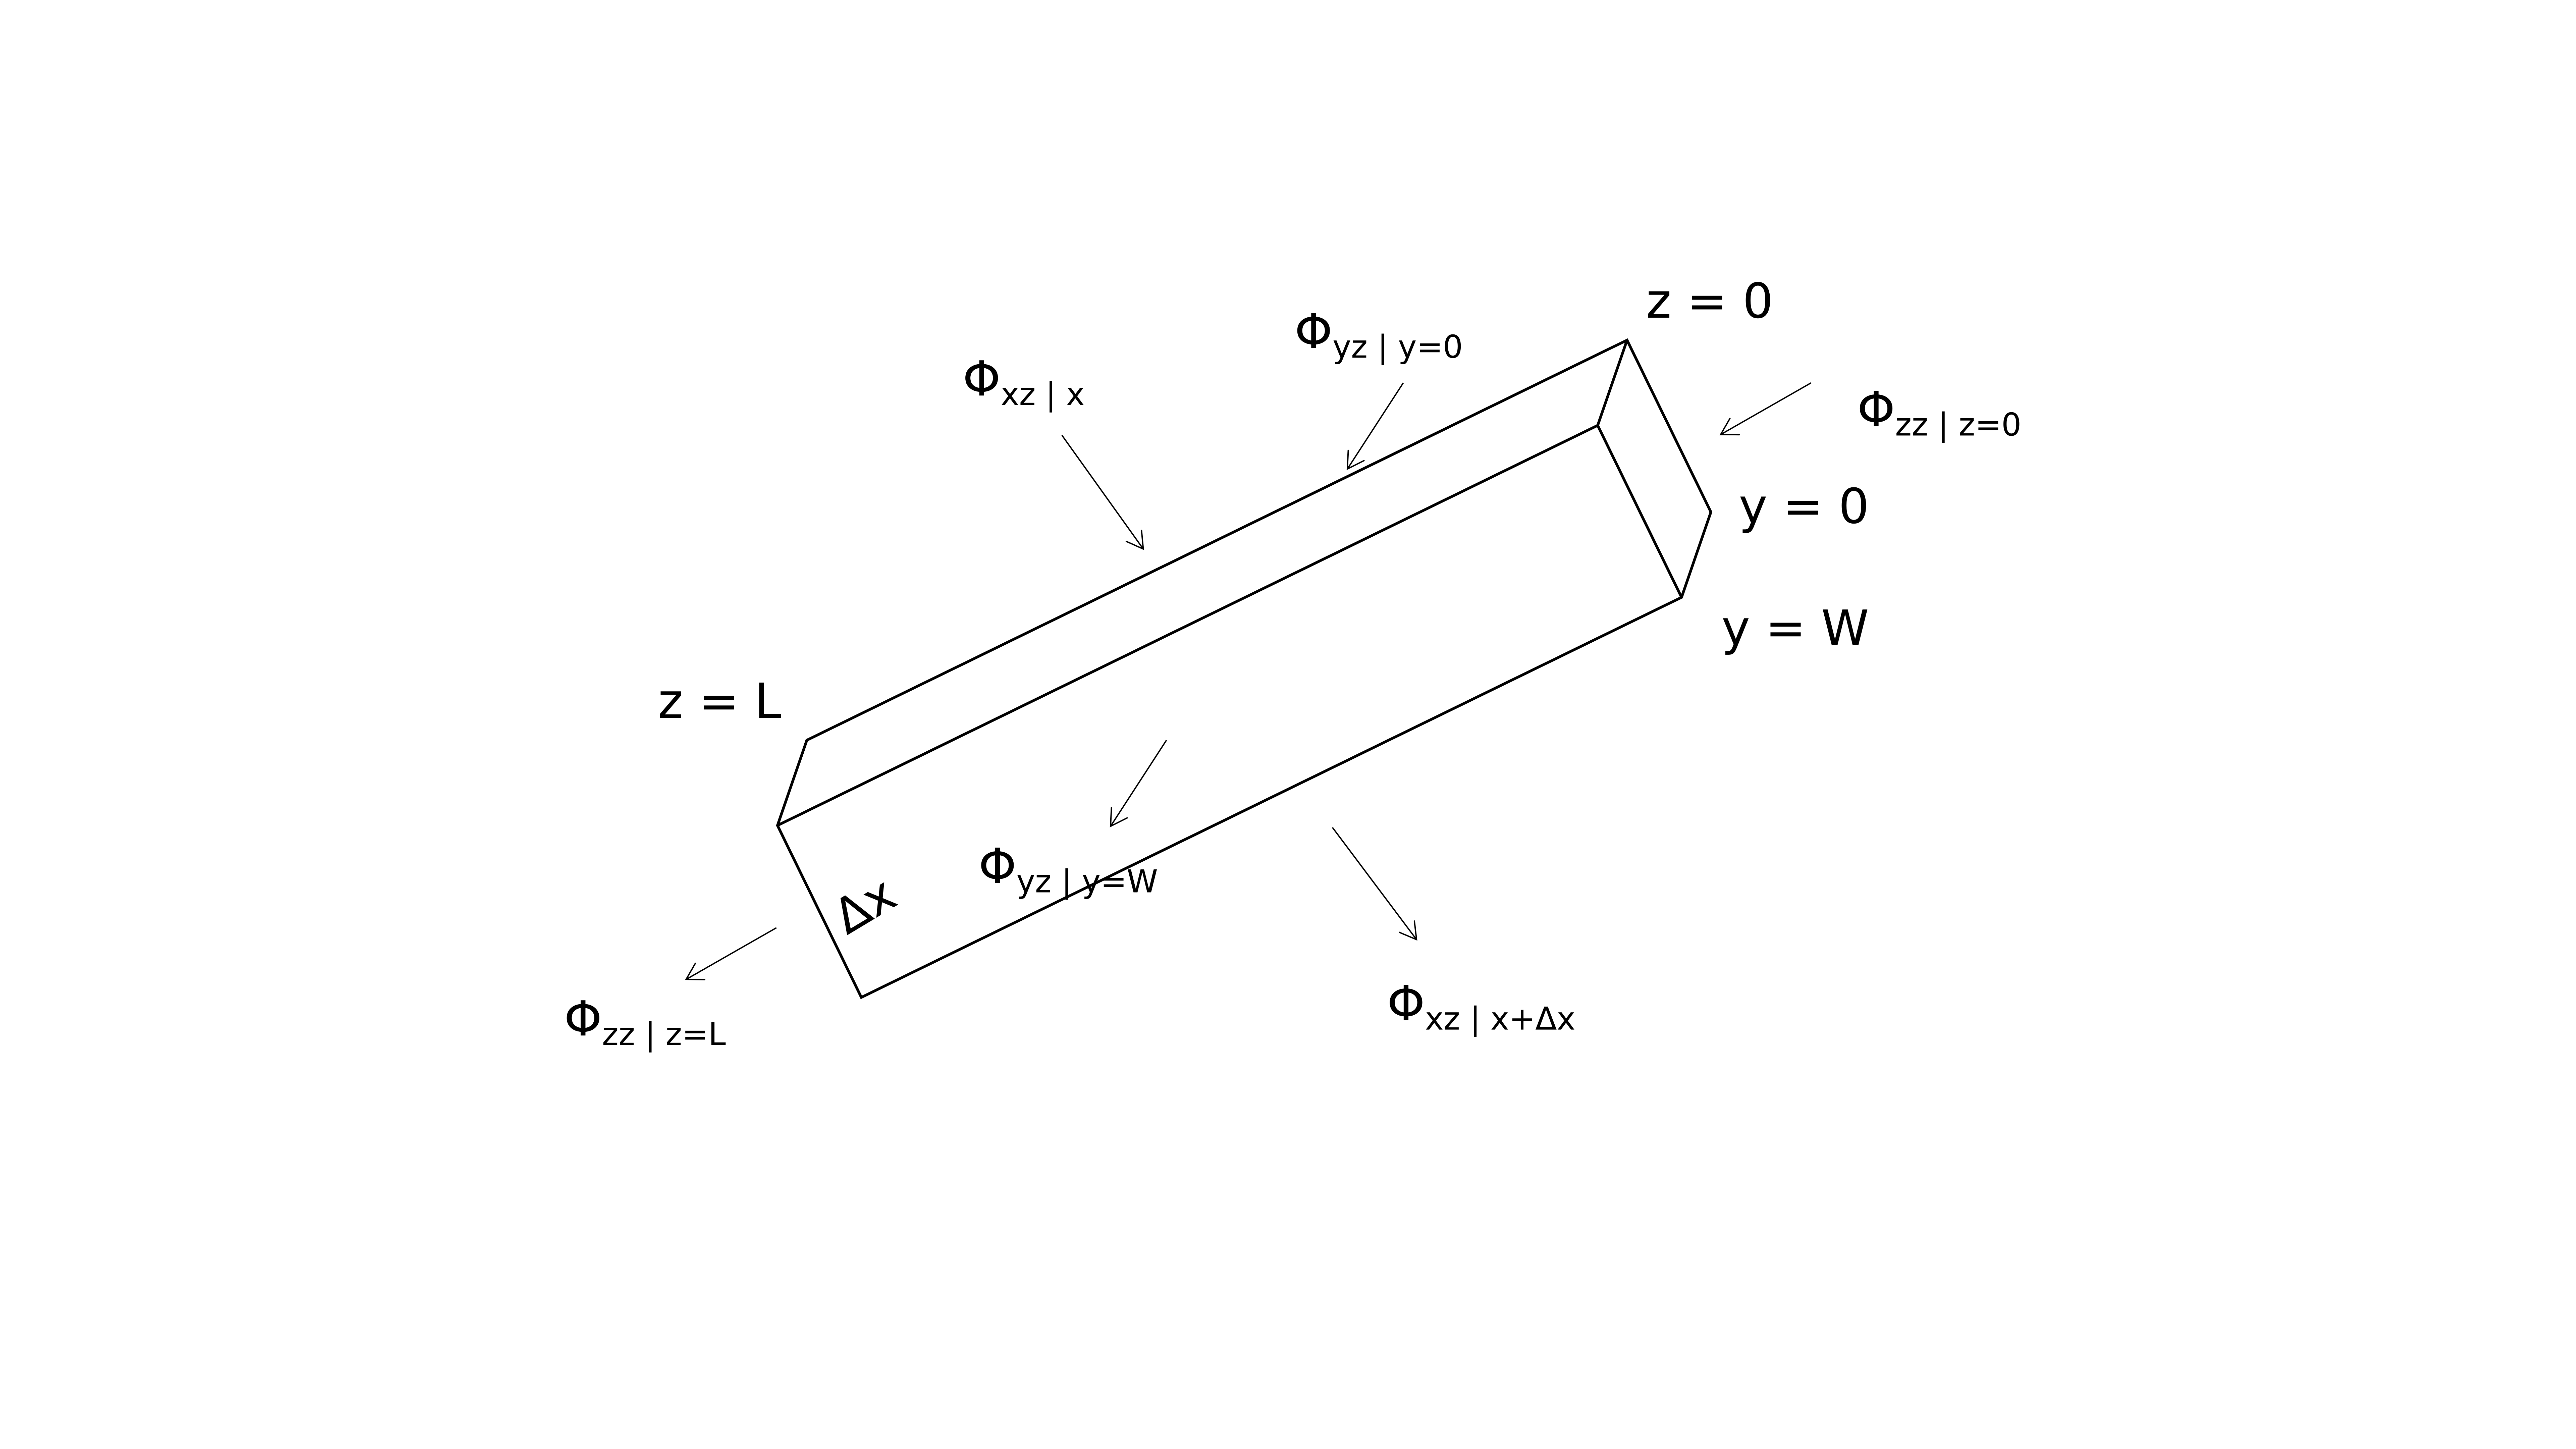
\includegraphics[scale=0.07]{shell_mom.png}
    \caption{Shell momentum terms for the falling film}
\end{figure}


Now, let us actually carry out the momentum balance:

\begin{itemize}

    \item \{Rate of momentum in across surface z = 0\} + \{ " out at surface z = L\} + \{ " in at surface x = x\} + \{ " out at surface x = x $+ \Delta$ x \} + \{ " in at surface y = 0\} + \{ " out at surface y = W\} + \{Force of gravity\} = 0

    \item Rate of momentum in across a surface is given by (Area of that surface) $\times$ (Momentum flux across the same surface).

    \item Consider the rate of momentum in across surface z = 0. This is given by (Area parallel to xy plane) $\times \phi_{zz|z=0}$ = $(W \Delta x) \times \phi_{zz|z=0}$.

    \item The rate of momentum out at surface x = x + $\Delta$ x is similarly $(WL) \phi_{xz|x+\Delta x}$. Since the area parallel to the yz plane is WL. 
        
    \item Similarly the area parallel to the xz plane is $L \Delta x$ amd can be used to see the z-momentum imparted to the shell in the y direction.

    \item The force of gravity is $M_{shell} g cos(\beta)$. The mass of the shell is given by (Density) $\times$ (Shell Volume) = $\rho \times (WL\Delta x)$.

    \item The final shell momentum expression is : $$(W\Delta x) \times (\phi_{zz|z=0} - \phi_{zz|z=L}) + (WL)\times(\phi_{xz|x=x} - \phi_{xz|x=x+\Delta x}) + (L\Delta x)\times(\phi_{yz|y=0} - \phi_{yz|y=W}) + \rho g cos(\beta) \times (WL \Delta x) = 0$$

    \item Divide this expression by $WL\Delta x$ to get $$\frac{\phi_{zz|z=0} - \phi_{zz|z=L}}{L} + \frac{\phi_{xz|x=x} - \phi_{xz|x=x+\Delta x}}{\Delta x} + \frac{\phi_{yz|y=0} - \phi_{yz|y=W}}{W} + \rho g cos(\beta) = 0$$
        
    \item From the above expansions, we can see that since $v_{y} = v_{x} = 0$ and since $\frac{\partial v_{z}}{\partial y} = 0$, that this equation reduces to simply the x term and the gravity term. In the x term $\phi_{xx} = \tau_{xx}$ since $v_{x}$ is 0.

    \item Taking the limit of shell thickness tending to 0, the x term reduces as such : $$\lim_{\Delta x \to 0} \frac{\tau_{xz|x=x} - \tau_{xz|x=x+\Delta x}}{\Delta x} = \frac{\partial \tau_{xz}}{\partial x}$$


    \item The final expression is: $$\frac{\partial \tau_{xz}}{\partial x} = \rho g cos(\beta)$$. This is our first-order differential equation in $\tau$. 

    \item Integrate this differential equation to get the shear stress profile : $\tau_{xz} = (\rho g cos(\beta)) x + C_{1}$, where $C_{1}$ is a constant of integration.

    \item To get $C_1$ apply the boundary condition. At the liquid-air interface (x=0), no momentum is imparted, i.e. $\tau_{xz|x=0} = 0$. Hence we derive that $C_1 = 0$.

    \item Now to get the velocity profile, substitute Newton's law of viscosity into the shear stress expression. $\tau_{xz} = -\mu \frac{d v_{z}}{dx}$ to get : $$-\mu \frac{dv_{z}}{dx} = \rho g cos(\beta) x$$.

    \item Integrating, we get $$v_{z} = -\frac{\rho g cos(\beta)}{2 \mu} x^{2} + C_{2}$$.

    \item Apply the no-slip boundary condition for the solid-fluid interface to get $C_{2}$. At $x = \delta, v_z = 0$. $$-\frac{\rho g cos(\beta)}{2 \mu} \delta^2 + C_{2} = 0$$.

    \item Substituting it back into the velocity expression, we get the final expression for the velocity to be $$v_{z} = \frac{\rho g cos(\beta)}{2 \mu} (\delta^2 - x^2)$$.

    \item There are some advantages to writing this in terms of a dimensionless variable, so we write $$v_{z} = \frac{\rho g \delta^2 cos(\beta)}{2 \mu} (1 - (\frac{x^2}{\delta^2}))$$.

\end{itemize}


% TODO : Add profile graphs, add sections on avg vel and film thickness


\subsubsection{Flow through a Cylindrical Tube}

Suppose we have a cylindrical tube of radius R and length L, held vertically and a fluid is flowing through it. The pressure at the top of the tube is $P_o$ and the pressure at the bottom is $P_L$. What is the velocity profile of the fluid flowing through the tube?

% TODO : Insert diagram of system and shell

\begin{itemize}
    \item This problem must be dealt with in cylindrical coordinates. The directions of interest hence are $r, \theta, z$. Problem domain is $z \in [0, L] , r \in [0, R], \theta \in [0, 2\pi]$.

    \item Assume that the flow is laminar and steady-state, with constant fluid viscosity and density. This immediately means there is no variation of velocities across the axial direction.

    \item Furthermore, we assume that the flow is only because of gravity and pressure difference. Which means the fluid is only flowing downwards. The radial and angular components of velocity hence become 0. $v_r = 0, v_{\theta} = 0$. In combination with the previous point, we also infer that $v_z$ is only a function of r and not $\theta$ or z.

    \item To apply shell momentum balances, we need to understand how our momentum of interest propagates along the direction of interest. In this case it is z-momentum in radial direction.

    \item Hence, we consider a thin cylindrical shell concentric to the cylinder and balance momentum across it.

    \item The momentum balance equation across this shell is : \{Rate of momentum in across surface z = 0\} + \{ " out at surface z = L\} + \{ " in at surface r = r\} + \{ " out at surface r = r $+ \Delta$ r \} + \{Force of Gravity\} = 0

    \item Rate of momentum in across a surface is given by (Area of that surface) $\times$ (Momentum flux across the same surface).

    \item Consider the rate of momentum in across surface z = 0. This is given by $(2 \pi r \Delta r) \times \phi_{zz|z=0}$.

    \item The rate of momentum out at surface r = r + $\Delta$ r is similarly $(2 \pi r l) \phi_{rz|r+\Delta r}$. 

    \item The force of gravity is $M_{shell} g$. The mass of the shell is given by (Density) $\times$ (Shell Volume) = $\rho \times (2 \pi r l \Delta r)$.

    \item The final shell momentum expression is : $$(W\Delta x) \times (\phi_{zz|z=0} - \phi_{zz|z=L}) + (WL)\times(\phi_{xz|x=x} - \phi_{xz|x=x+\Delta x}) + (L\Delta x)\times(\phi_{yz|y=0} - \phi_{yz|y=W}) + \rho g cos(\beta) \times (WL \Delta x) = 0$$

    \item Divide this expression by $WL\Delta x$ to get $$\frac{\phi_{zz|z=0} - \phi_{zz|z=L}}{L} + \frac{\phi_{xz|x=x} - \phi_{xz|x=x+\Delta x}}{\Delta x} + \frac{\phi_{yz|y=0} - \phi_{yz|y=W}}{W} + \rho g cos(\beta) = 0$$
        
    \item From the above expansions, we can see that since $v_{y} = v_{x} = 0$ and since $\frac{\partial v_{z}}{\partial y} = 0$, that this equation reduces to simply the x term and the gravity term. In the x term $\phi_{xx} = \tau_{xx}$ since $v_{x}$ is 0.

    \item Taking the limit of shell thickness tending to 0, the x term reduces as such : $$\lim_{\Delta x \to 0} \frac{\tau_{xz|x=x} - \tau_{xz|x=x+\Delta x}}{\Delta x} = \frac{\partial \tau_{xz}}{\partial x}$$


     

\end{itemize}



\subsubsection{Narrow Slit and Couette Flow}

\section{Shell Energy Balances}

In this section, we will try to obtain the following for various geometries:

\begin{itemize}

    \item Temperature profiles.

    \item Heat flux profiles ($q_{i}$)

    \item Maximum temperature and average temperature.

\end{itemize}


The energy balance equation across a thin shell is as such:

\{Rate of energy in by conduction and convection\} - \{Rate of energy outby conduction and convection\} + \{Rate of work done by molecular transport on the system\} - \{Rate of work done by molecular transport by the system\} + \{Rate of energy production\} + \{Rate of work done by external sources\} = 0

\subsection{Shell Energy Balance Algorithm:}

The shell energy balance procedure is very similar to the shell momentum balance procedure.

\begin{enumerate}

    \item \textbf{Identify non-vanishing terms} 
    
    \item \textbf{Write the energy balance over a thin shell perpendicular to spatial variables}

\item \textbf{Thickness of the shell tending to zero:} This derives the equation in terms of the energy flux.

    \item \textbf{Apply Fourier's Law of Heat Conduction:} This converts the energy flux expression into a first order differential equation in terms of temperature

    \item \textbf{Integrate and Apply Boundary Conditions:} This derives the temperature profile expression.


\end{enumerate}

\subsection{Boundary Conditions in Energy Transport}

\begin{itemize}

    \item Temperature at boundary maintained : For example, if a rod is attached to a heat bath of constant temperature (say, $200^{\circ}$ C) at one end, then the temperature of that end is fixed at $T(0) = 200$. (This is similar to a Dirichlet Boundary condition).

    \item Heat flux normal to a surface specified : $q(x=0) = -k \frac{dT}{dx}|_{x=0} = q_{0}$ (This is similar to a Neumann Boundary condition).

    \item Solid-Solid Interface : At the interface between two solids, we assume that the temperature at the interface is equal ($T_{I} = T_{II}$) and the heat flux is equal ($q_{I} = q_{II}$).

    \item Solid-Fluid Interface : The heat flux at the interface of a solid and a fluid is given by Newton's Law of cooling: $$q = h(T_{o} - T_{b})$$ Here $T_{o}$ is the surface temperature and $T_{b}$ is the bulk temperature of the fluid. h is the heat transfer coefficient.

\end{itemize}


\subsection{Illustrative Problems}

\subsubsection{Insulated Wire}

\subsubsection{Nuclear Heat Source}

\subsubsection{Viscous Heat Source}

\subsection{Free and Forced Convection Heat Transfer}


\section{Shell Mass Balances}

In this section, we will try to obtain the following for various geometries:

\begin{itemize}

    \item Concentration profiles.

    \item Mass flux profiles

\end{itemize}

The following is written in terms of mass and mass flux but conversion to molar flux is a simple exercise.

The mass balance equation is specified for a specific component A of the system. Across a thin shell, the conservation of mass of species A is given by :

\{Rate of mass of A in\} - \{Rate of mass of A out\} + \{Rate of mass of A produced or removed by homogeneous chemical reaction\} = 0

\subsection{Shell Mass Balance Algorithm:}

\begin{enumerate}

    \item \textbf{Identify non-vanishing terms} 
    
    \item \textbf{Write the mass balance over a thin shell perpendicular to spatial variables}

\item \textbf{Thickness of the shell tending to zero:} This derives the equation in terms of the mass flux.

    \item \textbf{Apply Fick's Law of Diffusion:} This converts the mass flux expression into a first order differential equation in terms of concentration.

    \item \textbf{Integrate and Apply Boundary Conditions:} This derives the concentration profile expression.


\end{enumerate}

\subsection{Boundary Conditions in Mass Transport}

\begin{itemize}

    \item Concentration at boundary maintained : $w_{A}(0) = w_{A,0}$ (This is similar to a Dirichlet Boundary condition).

    \item Mass flux normal to a surface specified : $n_{A}(x=0) = n_{A, 0}$ (This is similar to a Neumann Boundary condition).

    \item Surface : The mass flux at a surface is given by: $$n_{A, 0} = K_{c} (w_{A,0} - w_{A,b})$$. This is similar to Newton's law of cooling. Here $K_{c}$ is the mass transfer coefficient. $w_{A,0}$ is the surface concentration and $w_{A,b}$ is the concentration in the bulk of the fluid outside.

    \item Reaction : A chemical reaction can serve as a boundary condition if its rate at a surface is specified. $N_{A} = -k C_{A,0}$


\end{itemize}


\subsection{Illustrative Problems}

\subsubsection{Stagnant Gas Film}

\subsubsection{Homogeneous Chemical Reaction}

\subsubsection{Heterogeneous Chemical Reaction}
